
\documentclass[a4paper,12pt]{article} 
\usepackage[T2A]{fontenc}			
\usepackage[utf8]{inputenc}			
\usepackage[english,russian]{babel}	
\usepackage{amsmath,amsfonts,amssymb,amsthm,mathrsfs,mathtools} 
\usepackage{cancel}
\usepackage{multirow}
\usepackage[colorlinks, linkcolor = blue]{hyperref}
\usepackage{upgreek}\usepackage[left=2cm,right=2cm,top=2cm,bottom=3cm,bindingoffset=0cm]{geometry}
\usepackage{tikz}
\usepackage{graphicx}
\usepackage{subfig}
\usepackage{titletoc}
\usepackage{pgfplots}
\usepackage{xcolor}
\usepackage{wrapfig}
\author{Чекмарев И.Д.\\
Группа Б06-404}
\title{4.3.3. Исследование разрешающей способности микроскопа методом Аббе}
\date{}

%\begin{wrapfigure}{r}{0.5\textwidth}
%\begin{center}
%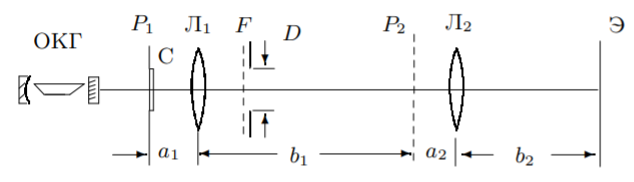
\includegraphics[width = 0.4\textwidth]{1.png}
%\end{center}
%\caption{}
%\end{wrapfigure}

%\begin{wrapfigure}{r}{0.5\textwidth}
%\begin{center}
%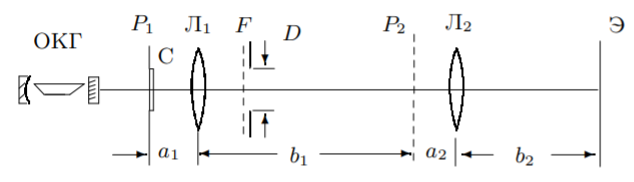
\includegraphics[width = 0.4\textwidth]{1.png}
%\end{center}
%\caption{}
%\end{wrapfigure}

\begin{document}
\maketitle
\textbf{Цель работы}: определение дифракционного предела разрешения объектива микроскопа.


\textbf{В работе используются}: лазер; кассета с набором сеток разного периода; щель с микрометрическим винтом; оптический стол с набором рейтеров и крепёжных винтов; экран; линейка.
\section*{Теория}
Для иммерсионного микроскопа разрешающая способность объектива при \textit{некогерентном} освещении
\begin{equation}
\ell_{min} \approx \dfrac{0.61\lambda}{n \sin u},
\end{equation}
где $u$ -- апертурный угол объектива микроскопа (угол между оптической осью и лучом, направленным из центра объекта в край линзы).

Метод Аббе для оценки разрешающей способности состоит в разделении хода хучей на две части: сначала рассматривается картина в задней фокальной плоскости $F$ объектива -- она называется \textit{первичным изображением} или \textit{фурье-образом}. Это первичное изображение рассматривается как источник волн (принцип Гюйгенса-Френеля), создающий изображение в плоскости $P_2$, сопряжённой плоскости предмета -- \textit{вторичное изображение}.\\
Первичное изображение есть картина дифракции Фраунгофера (на дифракционной решётке), если её период $d$, то для направления максимальной интенсивности $\varphi_m$
\begin{equation}
d \sin \varphi_m = m\lambda.
\end{equation}
При этом проходят пучки только с $\varphi_m < u$. Можно условием разрешения считать, что $u > \varphi_1$, иначе говоря
$$
\sin u \geq \lambda/d.
$$
или
\begin{equation}
d \geq \dfrac{\lambda}{\sin u} \approx \dfrac{\lambda}{D/2f},
\end{equation}
где $D$ -- диаметр линзы, $f$ -- фокусное расстояние.\\
Двумерную решётку можно рассматривать как две перпендикулярные друг другу, для максимумов которых выполняется соотношение
\begin{equation}
\begin{array}{c c}
d\sin \varphi_x = m_x \lambda, & d\sin \varphi_y = m_y \lambda. \\
\end{array}
\end{equation}
\newpage
\section*{Экспериментальная установка}
\begin{figure}[h]
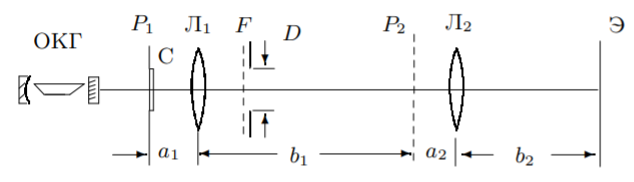
\includegraphics[scale=0.7]{1.png}
\centering
\caption{Схема установки.}
\end{figure}
Схема установки приведена на Рис. 1. Предметом $P_1$ служат сетки в кассете $C$. Линза $\text{Л}_1$ длиннофокусная, а $\text{Л}_2$ короткофокусная. В $F$ устанавливаются диафрагмы $D$, с помощью сеток с разными $d$ и щелевой диафрагмы можно проверить соотношение (3). Период сеток может быть измерен либо по расстоянию между дифракционными максимумами на экране, либо по увеличенному с помощью микроскопа изображению сетки на экране. Пространственную фильтрацию (получение наклонного изображение решётки) можно получить с помощью подбора угла наклона и ширины вспомогательной щели.
\newpage
\section*{Ход работы}
\subsection*{1. Определение периода решёток по их пространственному спектру}
Соберём установку согласно Рис 1, за исключением линз. Длина волны излучения лазера $\lambda = 532 \text{ нм}$.\\
Расстояние от сетки до экрана $H = 161 \pm 1 \text{ см}$, погрешность объясняется погрешностью меток на столе, использованных при измерении, и погрешностью прямого измерения.\\
Измерим линейкой на экране расстояние $\Delta x$ между $n+1$ максимумами и рассчитаем по формуле (2) с учётом $\varphi = \frac{\Delta x}{\sqrt{(H^2+\Delta x^2)}}$ период решётки $d = \frac{n \lambda}{\Delta x}\sqrt{(H^2+\Delta x^2)}$. Результаты приведены в Таблице 1.
\begin{table}[h]
\begin{tabular}{|c|c|c|c|c|c|}
\hline
Реш. & $2\Delta x$ см & $\sigma_{\Delta x}$, см & $2n$  & $d$, мкм & $\sigma_d$, мкм \\ \hline
1 верх     & 13.8         & 0.1                   & 2  & 12.4 & 0.2        \\ \hline
1 низ     & 13.8         & 0.1                   & 2  & 12.4 & 0.2        \\ \hline
2 верх     & 15.6         & 0.1                   & 6 & 33.0 &  0.4       \\ \hline
2 низ     & 5.5         & 0.1                   & 2 & 32 & 1 	\\ \hline
3 верх     & 8.3         & 0.1                   & 6 & 62 & 1        \\ \hline
3 низ     & 2.8         & 0.1                   & 2 & 61 & 3        \\ \hline
\end{tabular}
\centering
\caption{Периоды решёток, метод 1.}
\end{table}\\
Погрешность измерения $\Delta x$ -- цена деления линейки, $n$ -- один промежуток. Погрешность $d$ считаем по формуле
$$
\sigma_{d} = d\sqrt{\left(\dfrac{\sigma_{\Delta x}}{\Delta x}\right)^2 + \frac{1}{4}\left(4\left(\dfrac{\sigma_{\Delta x}}{\Delta x}\right)^2 + 4\left(\dfrac{\sigma_{H}}{H}\right)^2 \right)} = d\sqrt{2\left(\dfrac{\sigma_{\Delta x}}{\Delta x}\right)^2 + \left(\dfrac{\sigma_{H}}{H}\right)^2}
$$
\subsection*{2. Определение периода решёток по изображению, увеличинному с помощью микроскопа}
Соберём модель микроскопа, добавив линзы согласно Рис. 1. Фокусные расстояния линз $F_1 = 110 \text{ мм}$, $F_2 = 25 \text{ мм}$. Измеряем необходимые расстояния:
$$
\begin{array}{r}
a_1 = 140 \pm 10 \text{ мм},\\

a_2 + b_1 = 520 \pm 10 \text{  мм},\\
b_2 = 640 \pm 10 \text{ мм},
\end{array}
$$
Погрешности здесь обусловлены неточностями в положениях сеток и линз. Из формулы тонкой линзы $a_2 = \frac{b_2 F_2}{b_2 - F_2} = 26.02 \text{ мм}$, откуда $a_2 \approx F_2$, поэтому в дальнейшем будем использовать это значение, следовательно $b_1 = 495 \pm 10 \text{ мм}$. \\
Увеличение микроскопа $\Gamma = \dfrac{b_1 b_2}{a_1 a_2} = 90 \pm 7$. Погрешность находится по формуле
$$
\sigma_\Gamma = \Gamma\sqrt{\left(\dfrac{ \sigma a_1}{a_1}\right)^2 + \left(\dfrac{\sigma b_1}{b_1}\right)^2  + \left(\dfrac{\sigma b_2}{b_2}\right)^2}.
$$
Повторим измерения периодов изображений в новой конфигурации, погрешности считаются аналогично. Измерение представлены в Таблице 2.
\begin{table}[h]
\begin{tabular}{|c|c|c|c|c|c|}
\hline
Реш. & $2\Delta x$, см & $\sigma_{\Delta x}$, см & $2n$ & $d$, мкм & $\sigma_d$, мкм \\ \hline
1 верх     & 2.9            & 0.1      & 30  & 10.7       & 0.9               \\ \hline
1 низ    & 2.9           & 0.1      & 30  & 10.7       & 0.9               \\ \hline
2 верх    & 2.9           & 0.1     & 12  & 27       & 2               \\ \hline
2 низ    & 2.9           & 0.1      & 12  & 27     & 2              \\ \hline
3 верх    & 2.9           & 0.1     & 6  & 54     & 5              \\ \hline
3 низ     & 2.9           & 0.1     & 6  & 54      & 5              \\ \hline
\end{tabular}
\centering
\caption{Периоды решёток, метод 2.}
\end{table}\\
Здесь $d$ определялось по формуле $d = \dfrac{\Delta x}{\Gamma n}$, погрешность
$$
\sigma_d = d\sqrt{\left(\dfrac{\sigma \Delta x}{\Delta x}\right)^2  + \left(\dfrac{\sigma \Gamma}{ \Gamma}\right)^2}.
$$
Обратим внимание, что значения периодов верхних и нижних решёток совпадают.
\subsection*{3. Определение периода решёток по оценке разрешающей способности микроскопа}
Поместим в фокальной плоскости линзы $\text{Л}_1$ щелевую диафрагму с микрометрическим винтом и определим минимальную толщину $D$ при которой на экране видна двумерная решётка. В этом случае период будет вычисляться по формуле (3) в предельном случае
$$
d = \dfrac{2\lambda F_1}{D},
$$
погрешность вычисляется по формуле 
$$
\sigma_d = d \dfrac{\sigma_D}{D}.
$$
Результаты приведены в Таблице 3.
\begin{table}[h]
\begin{tabular}{|c|c|c|c|}
\hline
D, мм & $\sigma_D$, мм & $d$, мкм & $\sigma_d$, мкм \\ \hline
4.14  & 0.02           & 28.3    & 0.2            \\ \hline
2.190 & 0.010          & 53.0     & 0.3             \\ \hline
1.010 & 0.010          & 115.9    & 1.2             \\ \hline

\end{tabular}
\centering
\caption{Периоды решёток, метод 3.}
\end{table}\\
Через щель проходили только нулевой (по центру) и два первых максимумы, за исключением второй щели, где нулевой максимум был помещён к краю щели. Для первой решётки период таким методом измерить не получилось, так как ширины щели не хватает.
\newpage
\begin{figure}[h]
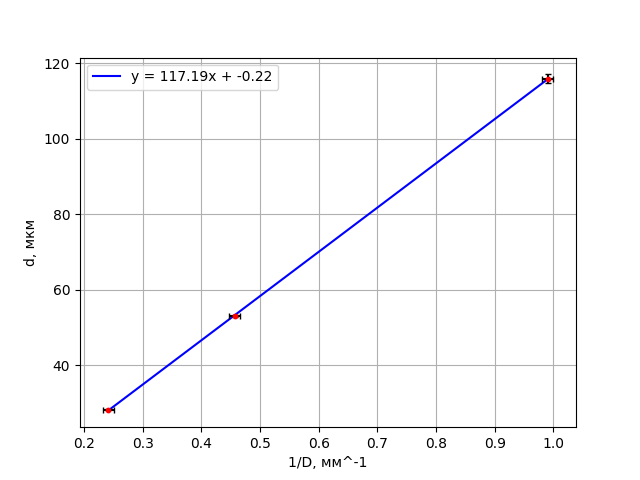
\includegraphics[scale=0.7]{Теория Аббе.png}
\centering
\caption{Зависимость $d = f(1/D)$.}
\end{figure}
Для проверки теории Аббе построим график $d = f(\frac{1}{D})$ со значениями $d$ из части 1, погрешность $\frac{1}{D}$ рассчитывается по формуле
$$
\sigma_{1/D} = \dfrac{\sigma_D}{D^2}.
$$
Угловой коэффициент прямой из МНК $k = (117.2 \pm 0.3) \cdot 10^{-9} \text{ м}^2$, в пределах погрешности он совпадает с теоретическим $2\lambda F_1 = 117 \cdot 10^{-9} \text{ м}^2$. Таким образом, теория Аббе подтвердилась.
\begin{table}[h]
\begin{tabular}{|c|c|c|c|c|}
\hline
Реш. & $1/D$, $\text{мм}^1$ & $\sigma_{1/D}$, $\text{мм}^1$ & $d$, мкм & $\sigma_d$, мкм \\ \hline
1    & 0.242               & 0.002              & 28.4       & 0.2               \\ \hline
2    & 0.457                & 0.003               & 53.6       & 0.2               \\ \hline
3    & 0.990                & 0.010               & 116      & 0.3               \\ \hline

\end{tabular}
\centering
\caption{Значения для графика $d = f(1/D)$.}
\end{table}
\newpage
\subsection*{4. Пространственная фильтрация и мультиплицирование}
Для наблюдения фильтрации на сетке 2 откроем щель так, чтобы она пропускала только максимум нулевого порядка и, поворачивая щель, наблюдаем за изменением картины. Картины представлены на Рис 3.
\begin{figure}[h]
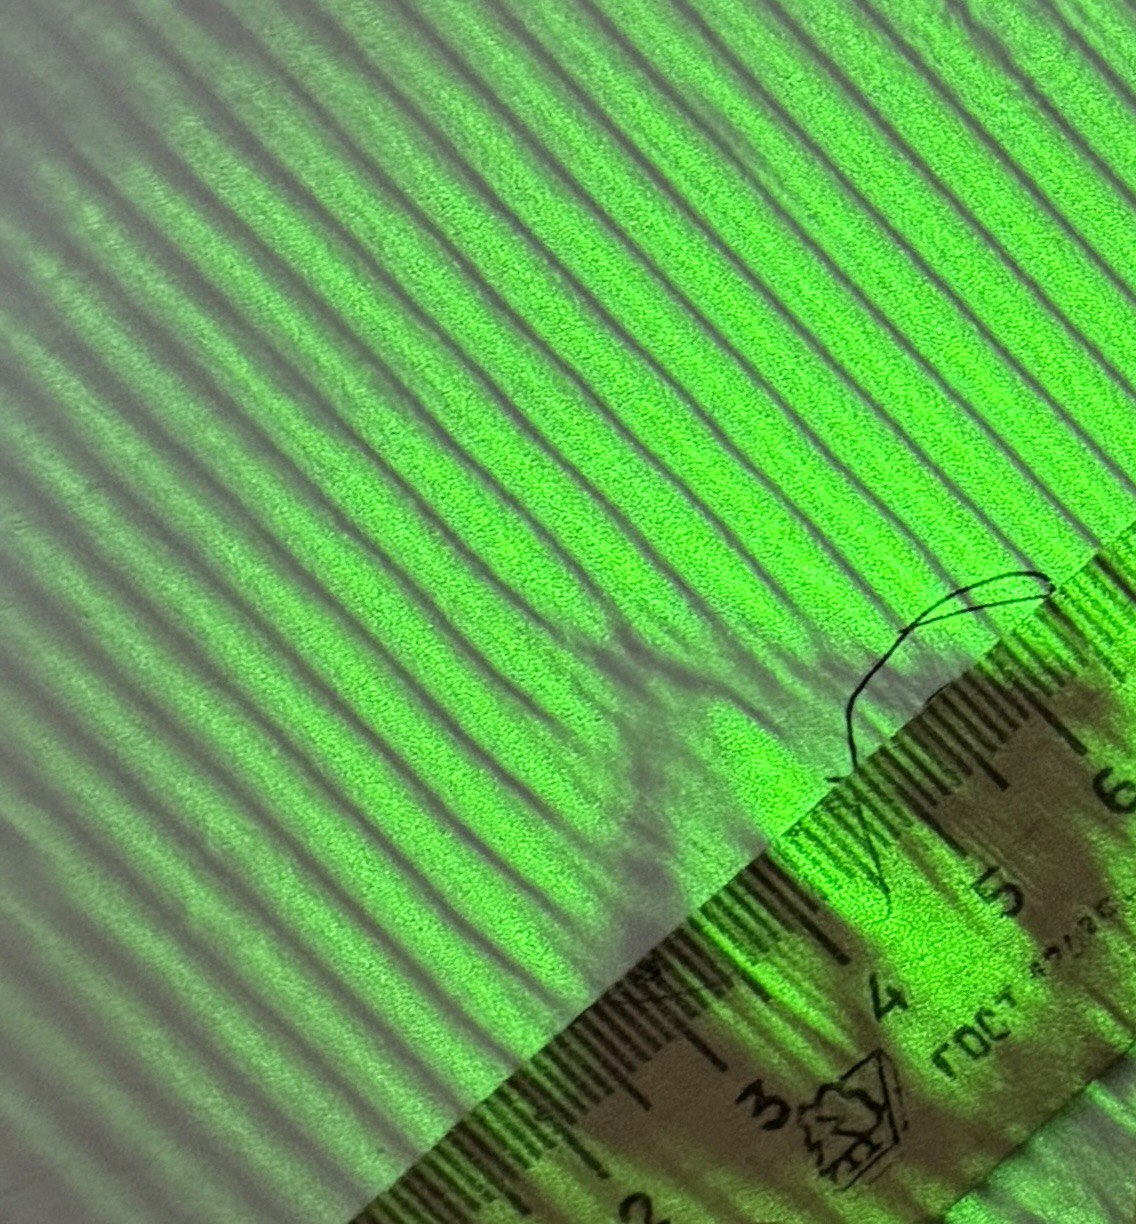
\includegraphics[scale=0.20]{diag.jpg}
\centering
\caption{ щель на $45^\circ (\frac{\pi}{4})$ ($m_x = m_y$)}
\end{figure}\\
Для наблюдения мультиплицированния поменяем местами сетку и щель, пронаблюлюдаем мультипликацию, картина представлена на Рис. 4.
\begin{figure}[h]
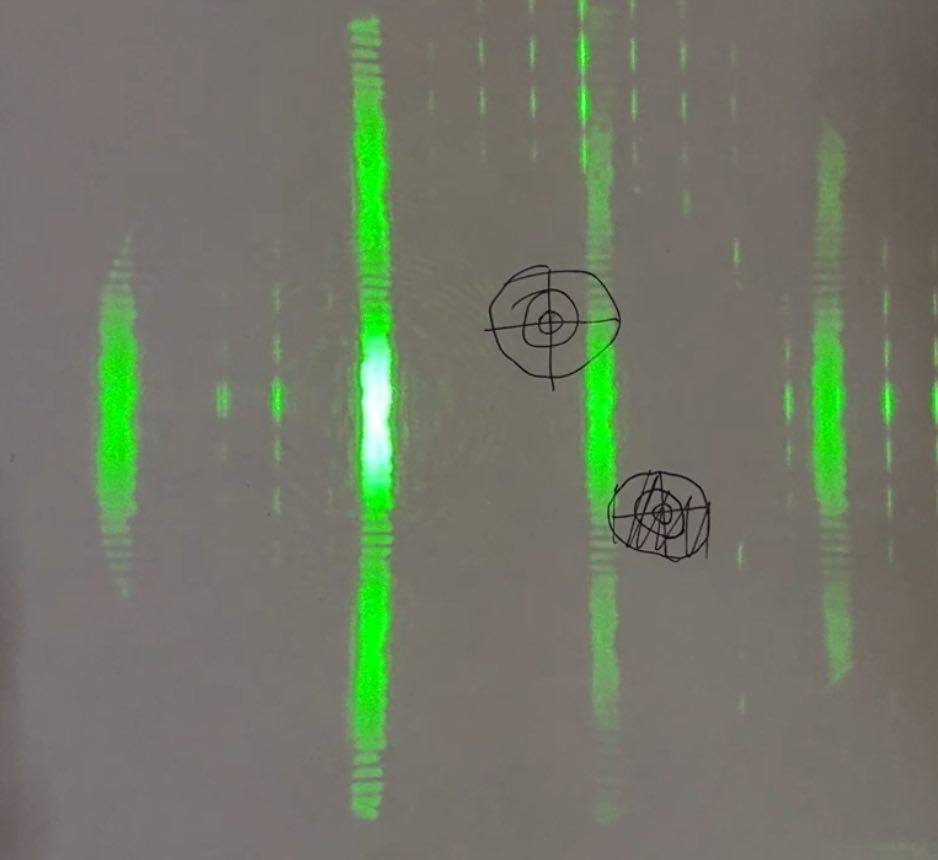
\includegraphics[scale=0.2]{mult.jpg}
\centering
\caption{Явление мультипликации.}
\end{figure}
\end{document}
